
\section{Vartiolaisten telttaretki 11.-13.4.}

% \smallskip
\noindent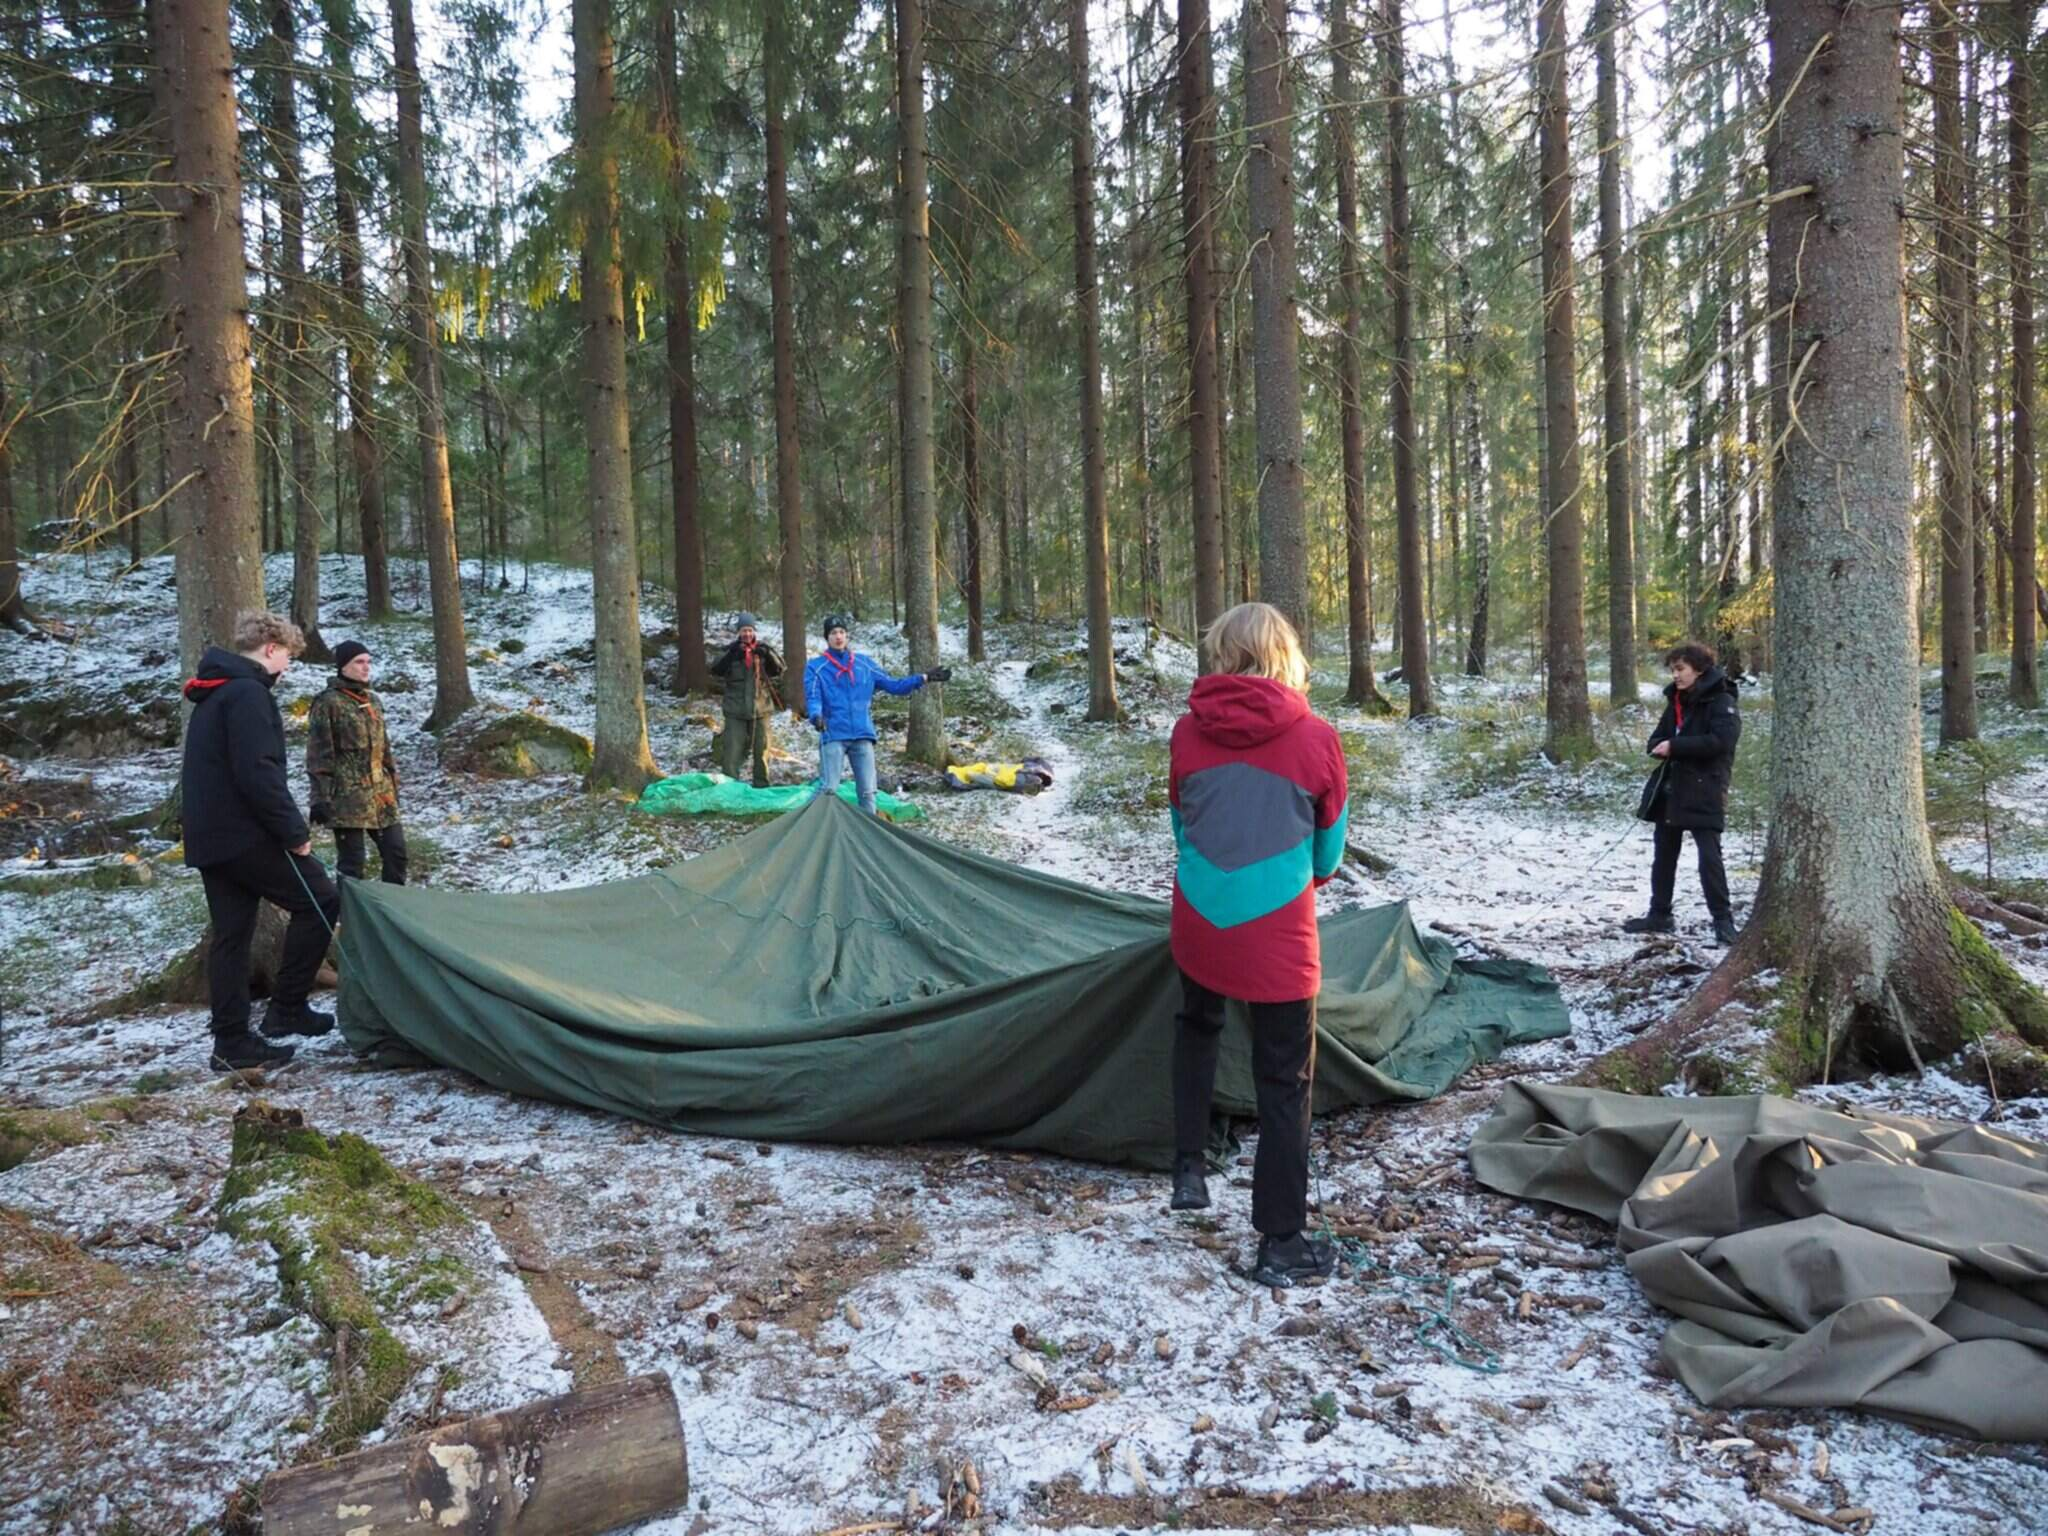
\includegraphics[width=1.0\linewidth]{assets/telttaretki4}

\begin{multicols}{2}

Huhtikuun yhdestoista päivä Kurkisuon rusakoiden seikkailijat ja tarpojat
lähtivät viileään mutta aurinkoiseen Sipoonkorpeen Bisajärven rannalle
telttailemaan ja suorittamaan kolmannen luokan riihitystä. Rusakot jakautuivat
Mikaelinkirkolla bussiosastoon sekä vanhaan tuttuun logistiikkaosastoon.
Leiriin ensimmäisenä saapui logistiikkaosasto puolijoukkueteltan, kamiinan ja
muiden varusteiden kanssa, vaikkei täysin selkeää parkkipaikkaa löytynytkään.
Hieman jäljessä saapui bussiosasto, joka väärään suuntaan mentyään ei ollut
huomannut parkkeerattua autoa.

Leiriin päästyään rusakot ryhtyivät pystyttämään puolijoukkuetelttaa,
hakkaamaan halkoja ja kaksi rusakoista pystytti oman pienemmän telttansa, koska
halusivat kokeilla sitä. Kun halot oli hakattu ja teltat kamiinaa myöten
pystytetty, menivät rusakot Bisajärven keittokatokselle syömään itse tuomiaan
iltapaloja. Kun rusakot saivat syötyä jaettiin yön kipinävuorot, minkä jälkeen
mentiin nukkumaan

\vspace*{-0.16cm}

\columnbreak

\begin{center}
	\noindent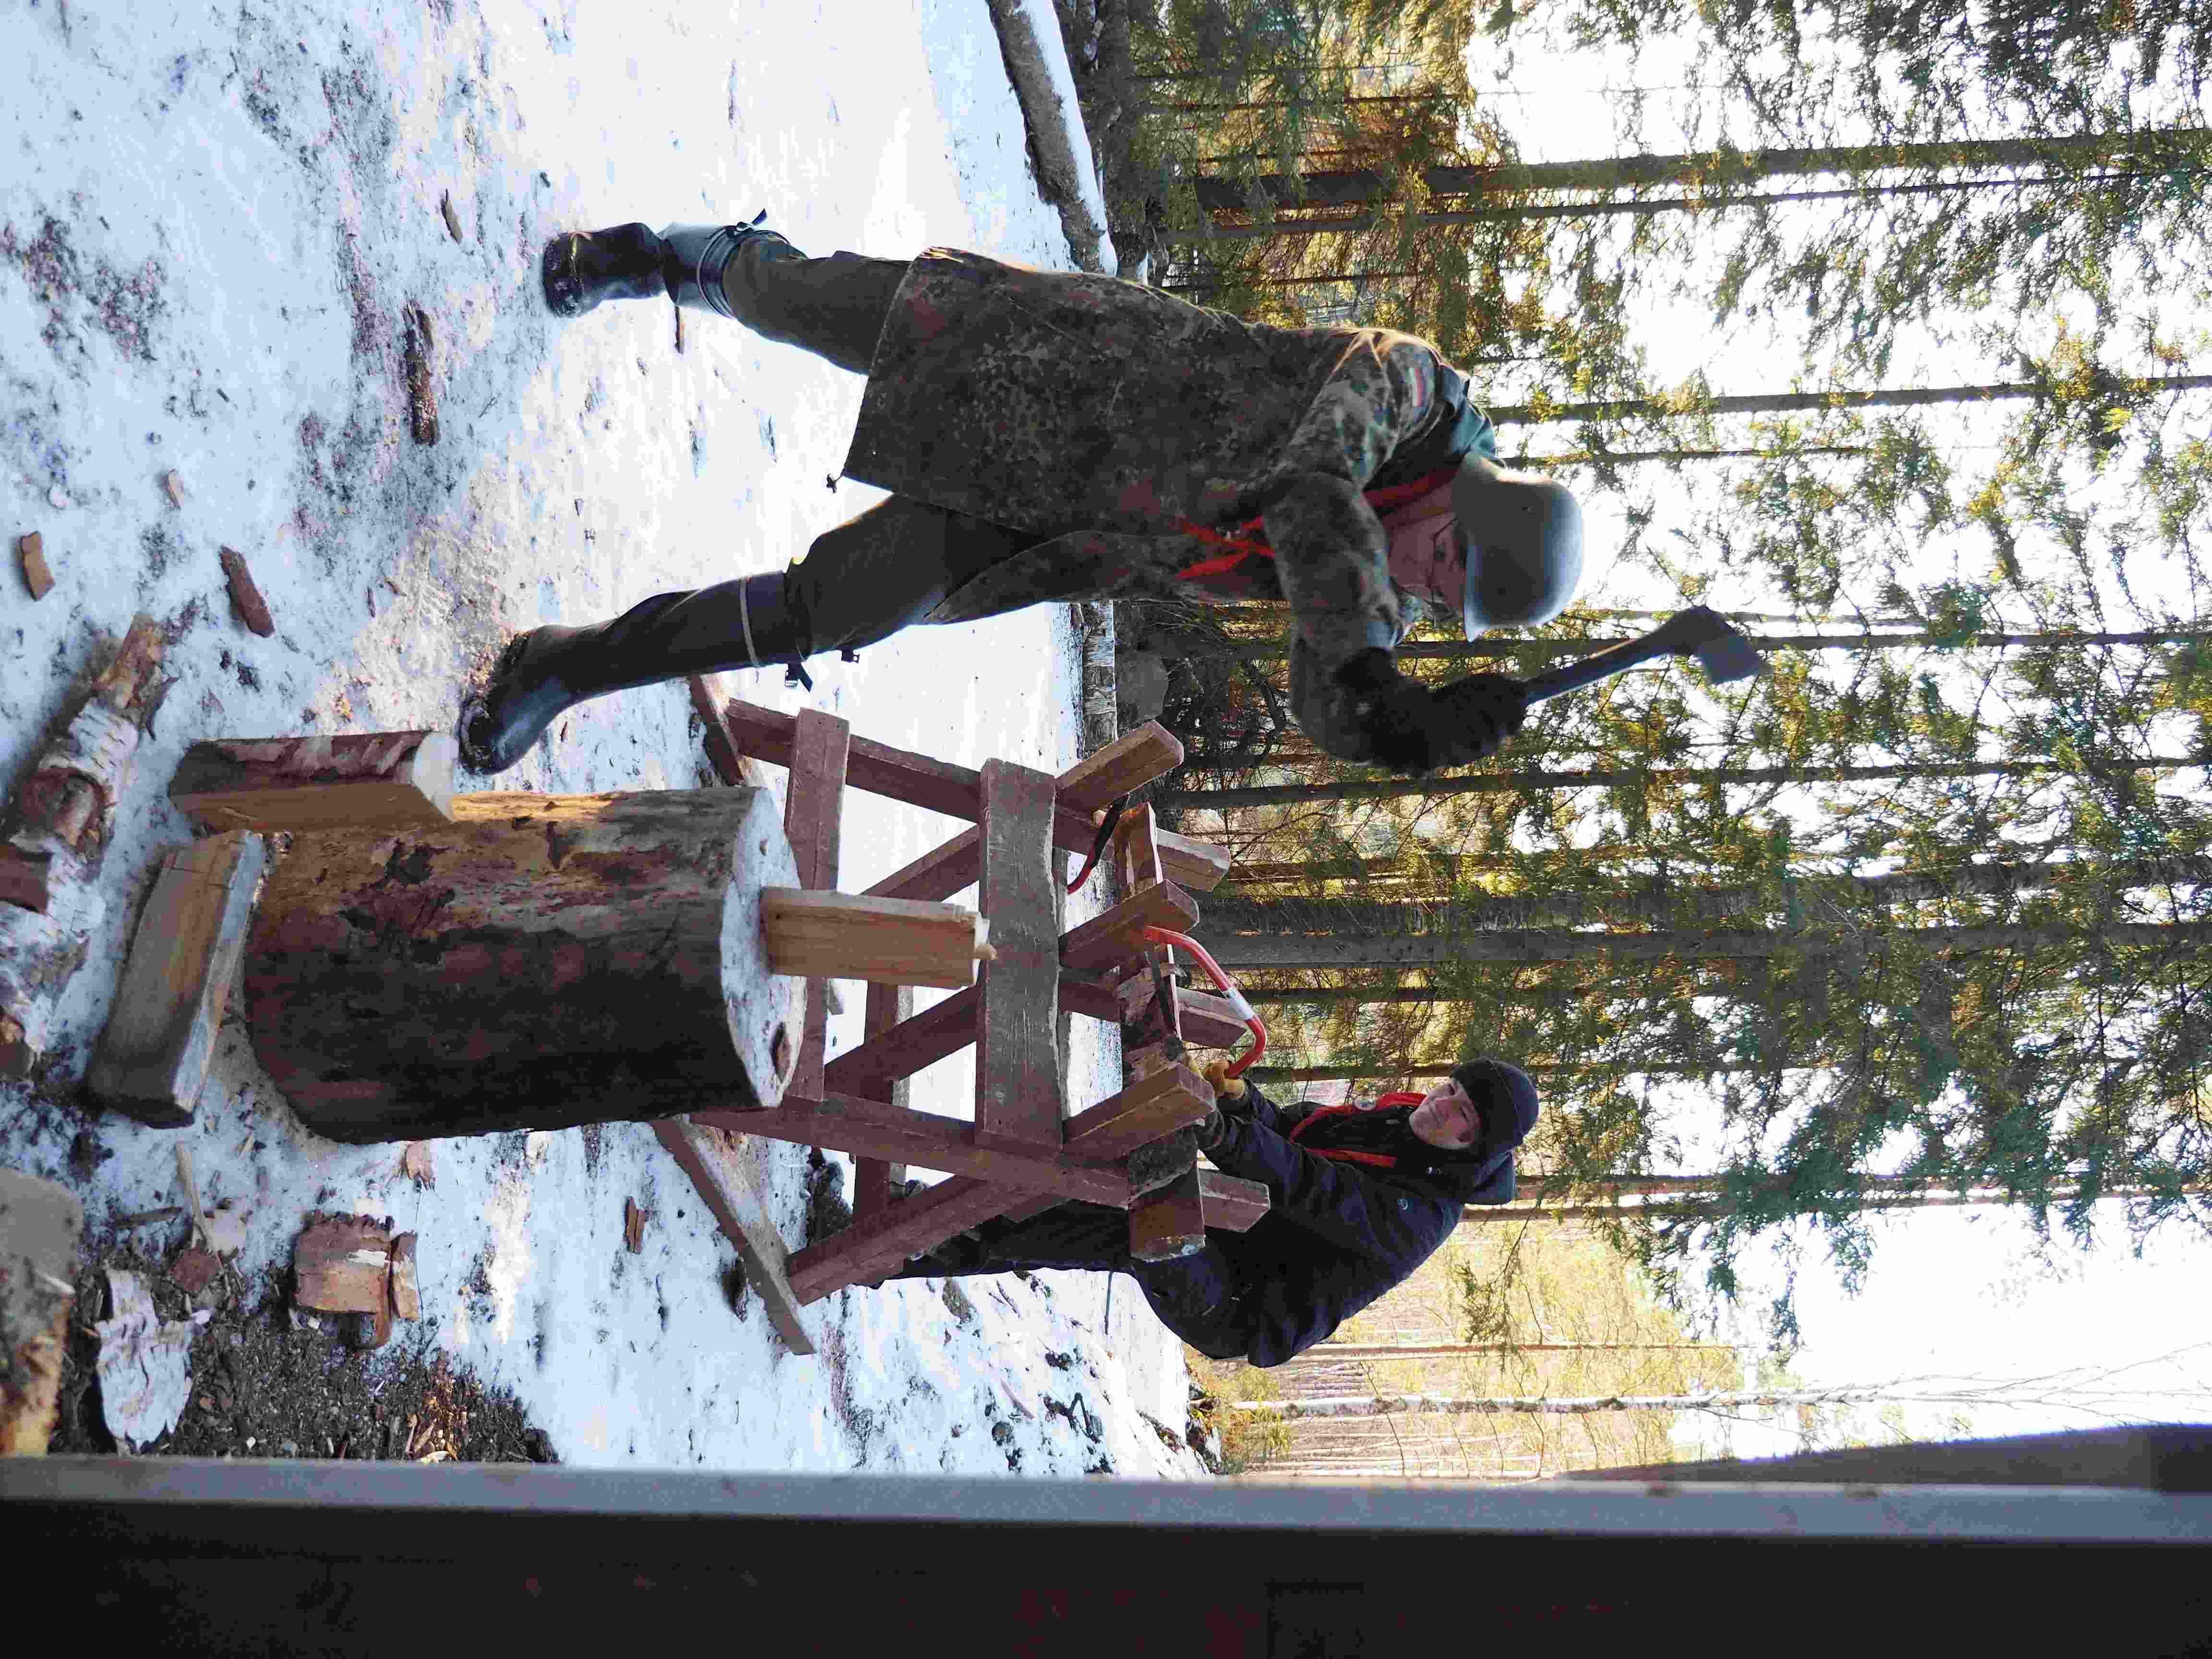
\includegraphics[height=0.9\linewidth,angle=90]{assets/telttaretki5}
\end{center}

Aamulla rusakot heräsivät lämpimälle aamupuurolle voisilmän, hillon tai
kuivattujen marjojen kera. Yön aikana oli satanut räntää, mistä huolimatta
molemmissa teltoissa oli nukuttu hyvin. Kun aamupala ja aamutoimet oli saatu
suoritettua, jaettiin vartiolaiset vartioihin ja niin saatiin riihitys
käyntiin.

Riihitys on vartioikäisten partio-ohjelmaan kuulunut suorite, joka toteutetaan
suunnistuksen muodossa. Tällä kertaa tehtävät alkoivat jo lähdöstä, jossa
vartiolaisten tehtävänä oli arvioida Bisajärven pisin halkaisija, rantaviivan
pituus sekä viereisen kukkulan korkeus järven pinnasta. Sieltä riihittäjät
suunnistivat ensimmäiselle rastille, jolla puhuttiin jokaisenoikeuksista,
eritoten tulenteosta ja siihen liittyvästä vastuusta. Toinen rasti oli
omistettu pillimerkeille, joita vartioiden tuli osata neljä kappaletta. Näihin
lukeutui esimerkiksi merkit jotka tarkoittavat “tulkaa tänne” ja “vaara.”
Kolmas rasti oli ensiapurasti, jossa riihittäjien tuli auttaa haavoittunutta
henkilöä. Neljäs rasti oli puhelinkentän ulottumattomissa oleva solmurasti.
Rastilla riihittäjien tuli tehdä merimies-, paalu- ja lippusolmu, sekä
siansorkka, ja tietää solmujen käyttötarkoitukset. Viimeisellä rastilla käytiin
läpi partioihanteita. Maalissa tehtävänä oli valmistaa vartioille lounaaksi
keittoa, josta tuli oikein hyvää ja se maistui kaikille.

\smallskip
\begin{center}
	\noindent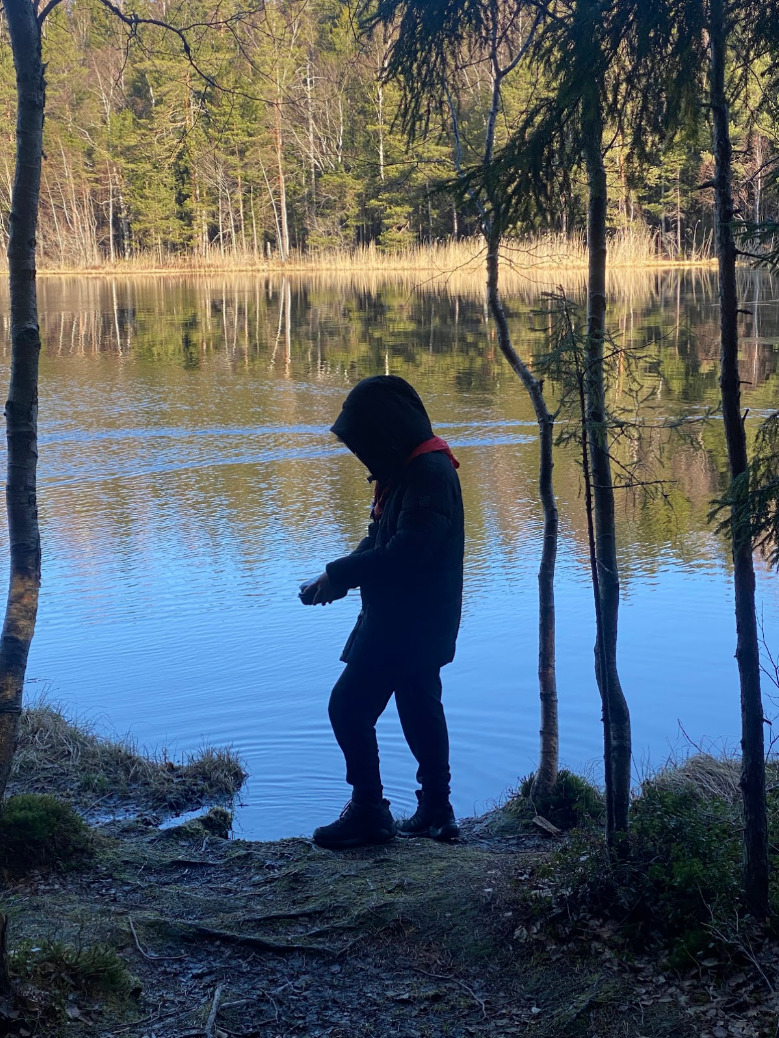
\includegraphics[width=0.9\linewidth]{assets/telttaretki1}
\end{center}

Lounaan jälkeen vartiot viimeistelivät riihityksen harjoittelemalla tulentekoa
sekä teltan kamiinalla, että risukeittimellä. Lopun iltapäivää rusakot
viettivät mitenkä halusivat, osa hakkasi halkoja ja osa vuoli makkaratikkuja,
joista muutamasta tuli hieman tarpeellista suurempia. 

\smallskip
\noindent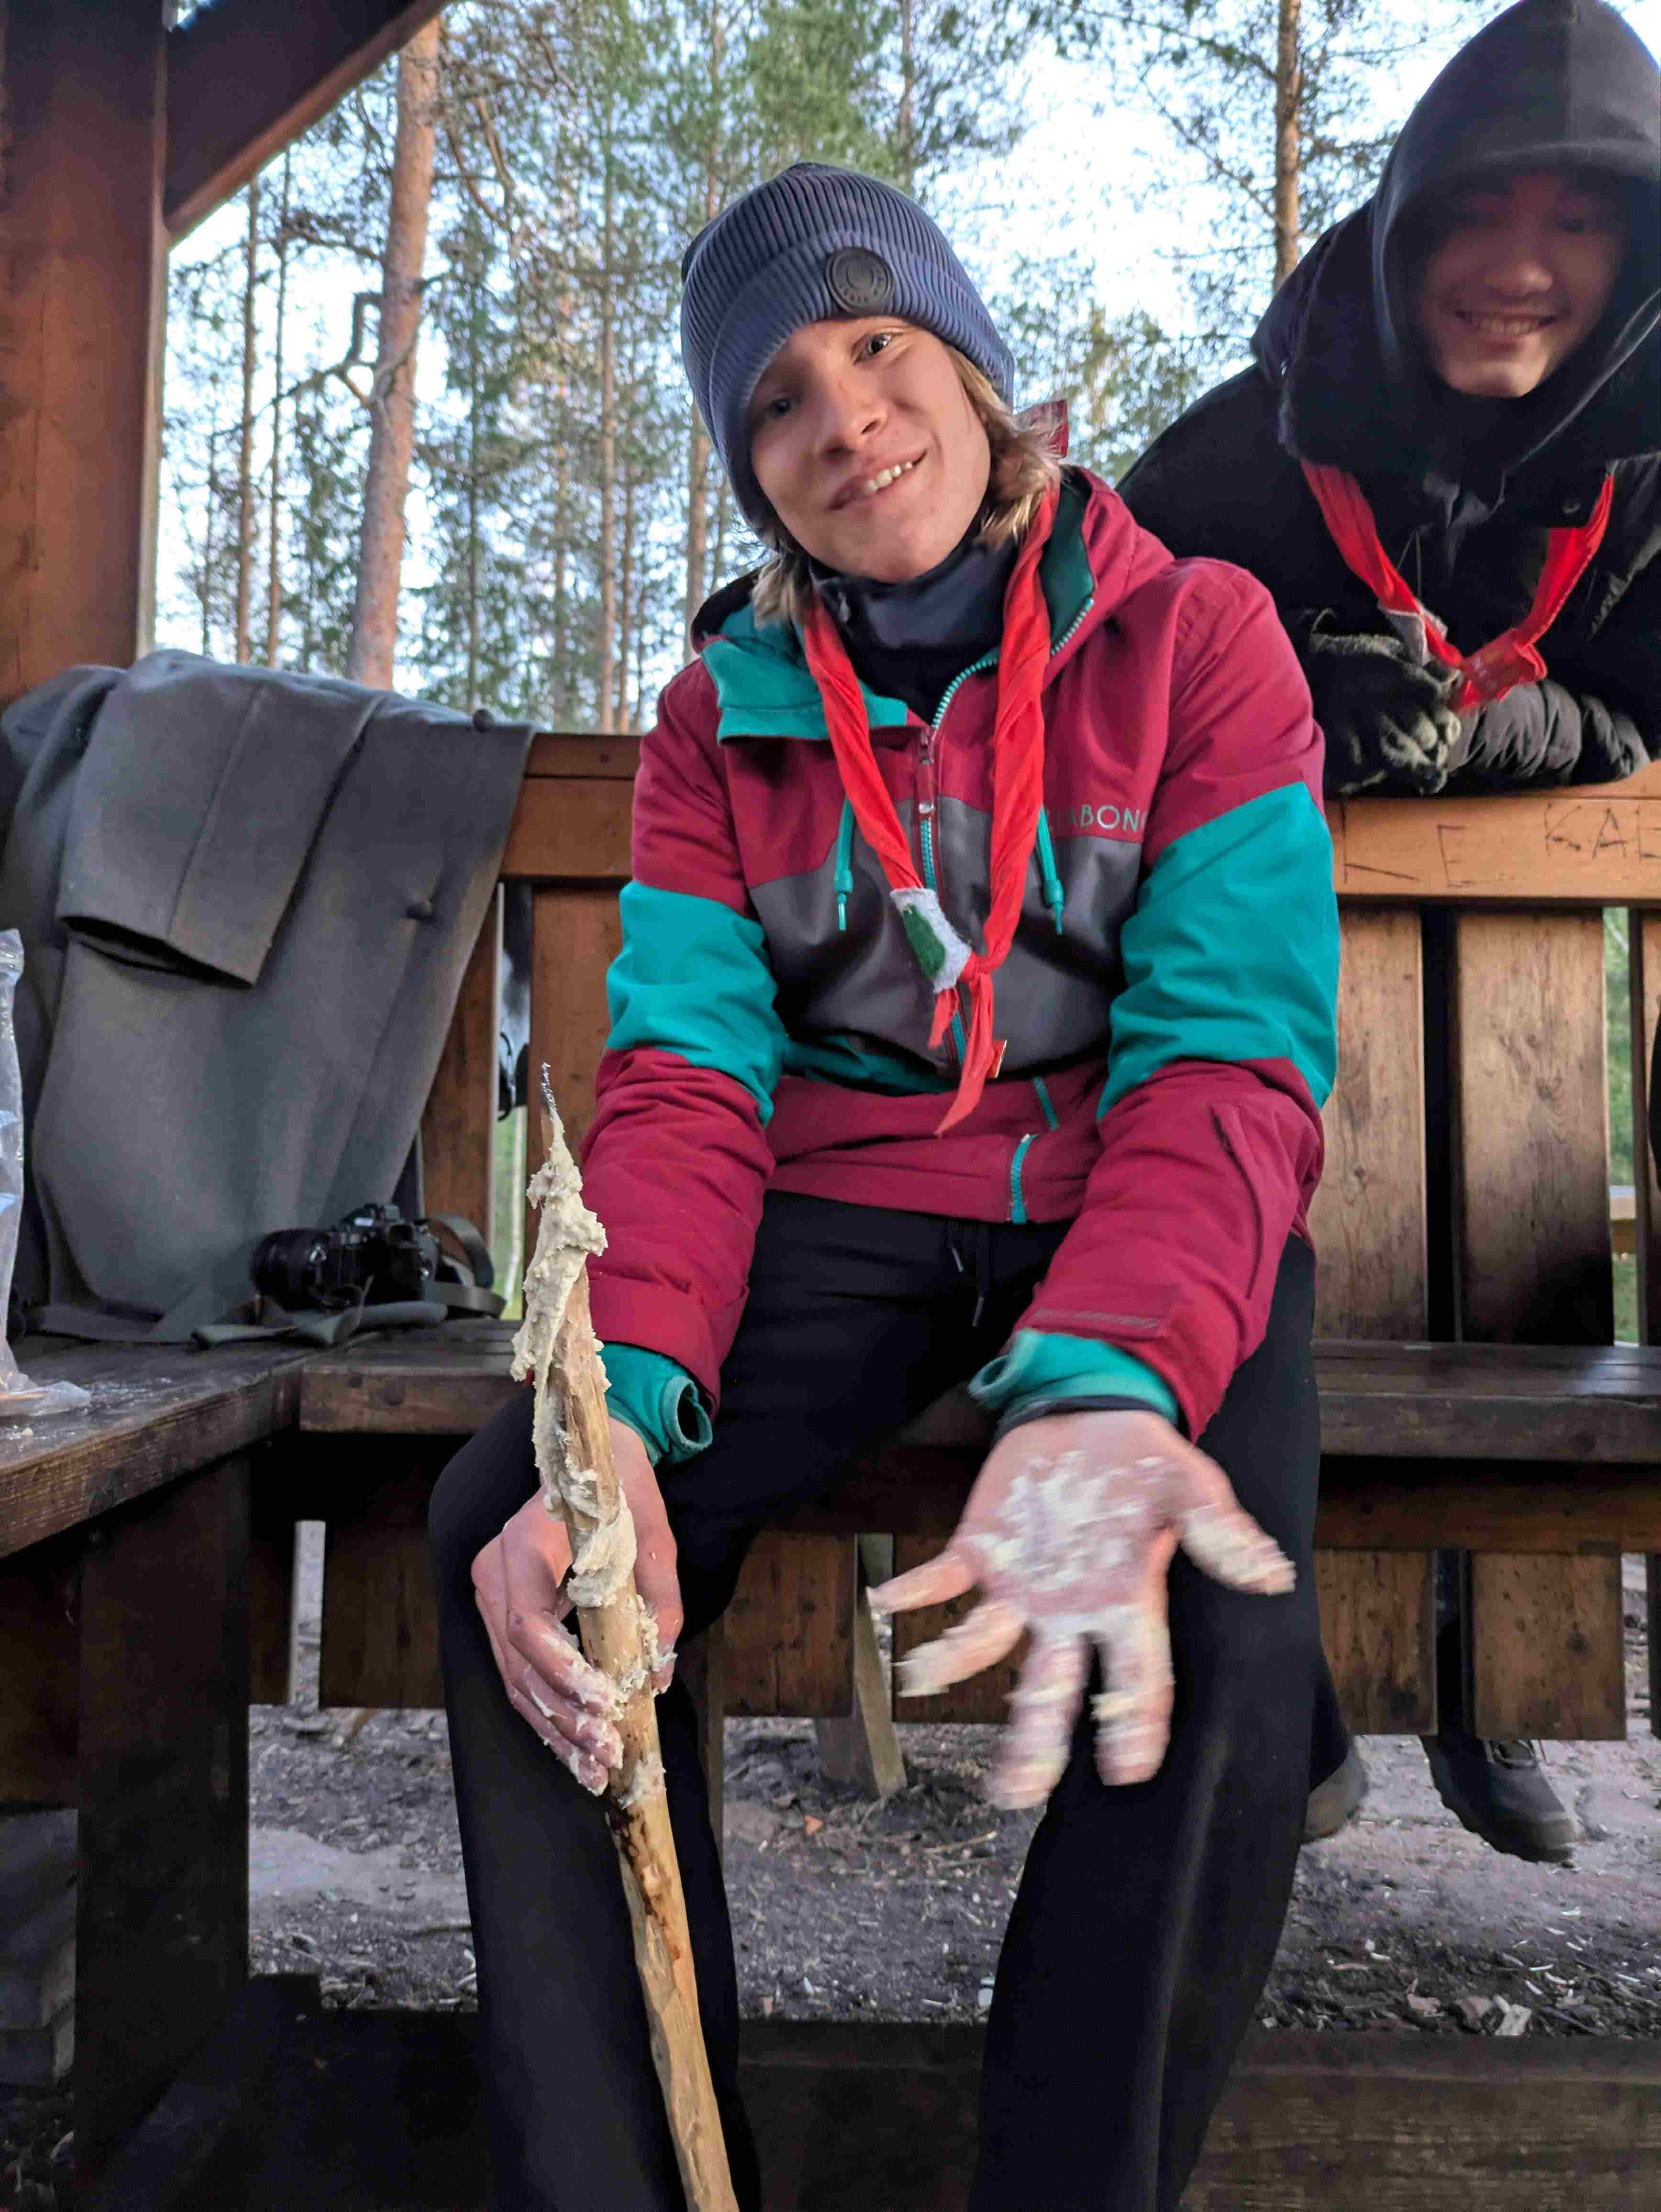
\includegraphics[width=1.0\linewidth]{assets/telttaretki3}

Makkaratikut vuoltuaan rusakot kokoontuivat jälleen keittokatokselle, jossa he
paistoivat makkaraa iltapalaksi. Makkaroiden jälkeen rusakot pääsivät myös
paistamaan tikkupullaa. Pullaa paistaessa taikina kierretään tikun ympäri, ja
paistetaan tulen yllä. Eräällä rusakolla paisto ei sujunut yhtä hyvin kun
taikina tarttui hänen käsiinsä. Iltapalan jälkeen osa rusakoista jäi vielä
keittokatokselle ihailemaan auringonlaskua, kunnes mentiin nukkumaan,

Sunnuntain vastaisena yönä kipinät sujuivat taas vaikeuksitta, mutta yöllä
leirin ohi kulki koira, joka haukkuessaan hämmästytti kipinässä olleita
rusakkoja. Sunnuntaina leirin purku aloitettiin herätyksen ja aamupalan
jälkeen. Pakatessa opeteltiin myös puolijoukkueteltan pakkaamista, joka
osoittautui osalle rusakoista oletettua vaikeammaksi. Loppujenlopuksi kaikki
saatiin pakattua, ja rusakot jakautuivat jälleen bussiosastoon sekä
logistiikkaosastoon. Logistiikkaosaston koko vahvuus eli seitsemän rusakkoa
survoutui alkumatkaksi yhteen autoon kaluston kanssa, jolloin muun muassa
rinkat kulkivat ensimmäiset kilometrit sylissä, kunnes osa rusakoista jätti
logistiikkaosaston ja hyppäsi bussiin kotia kohti.

\smallskip
\noindent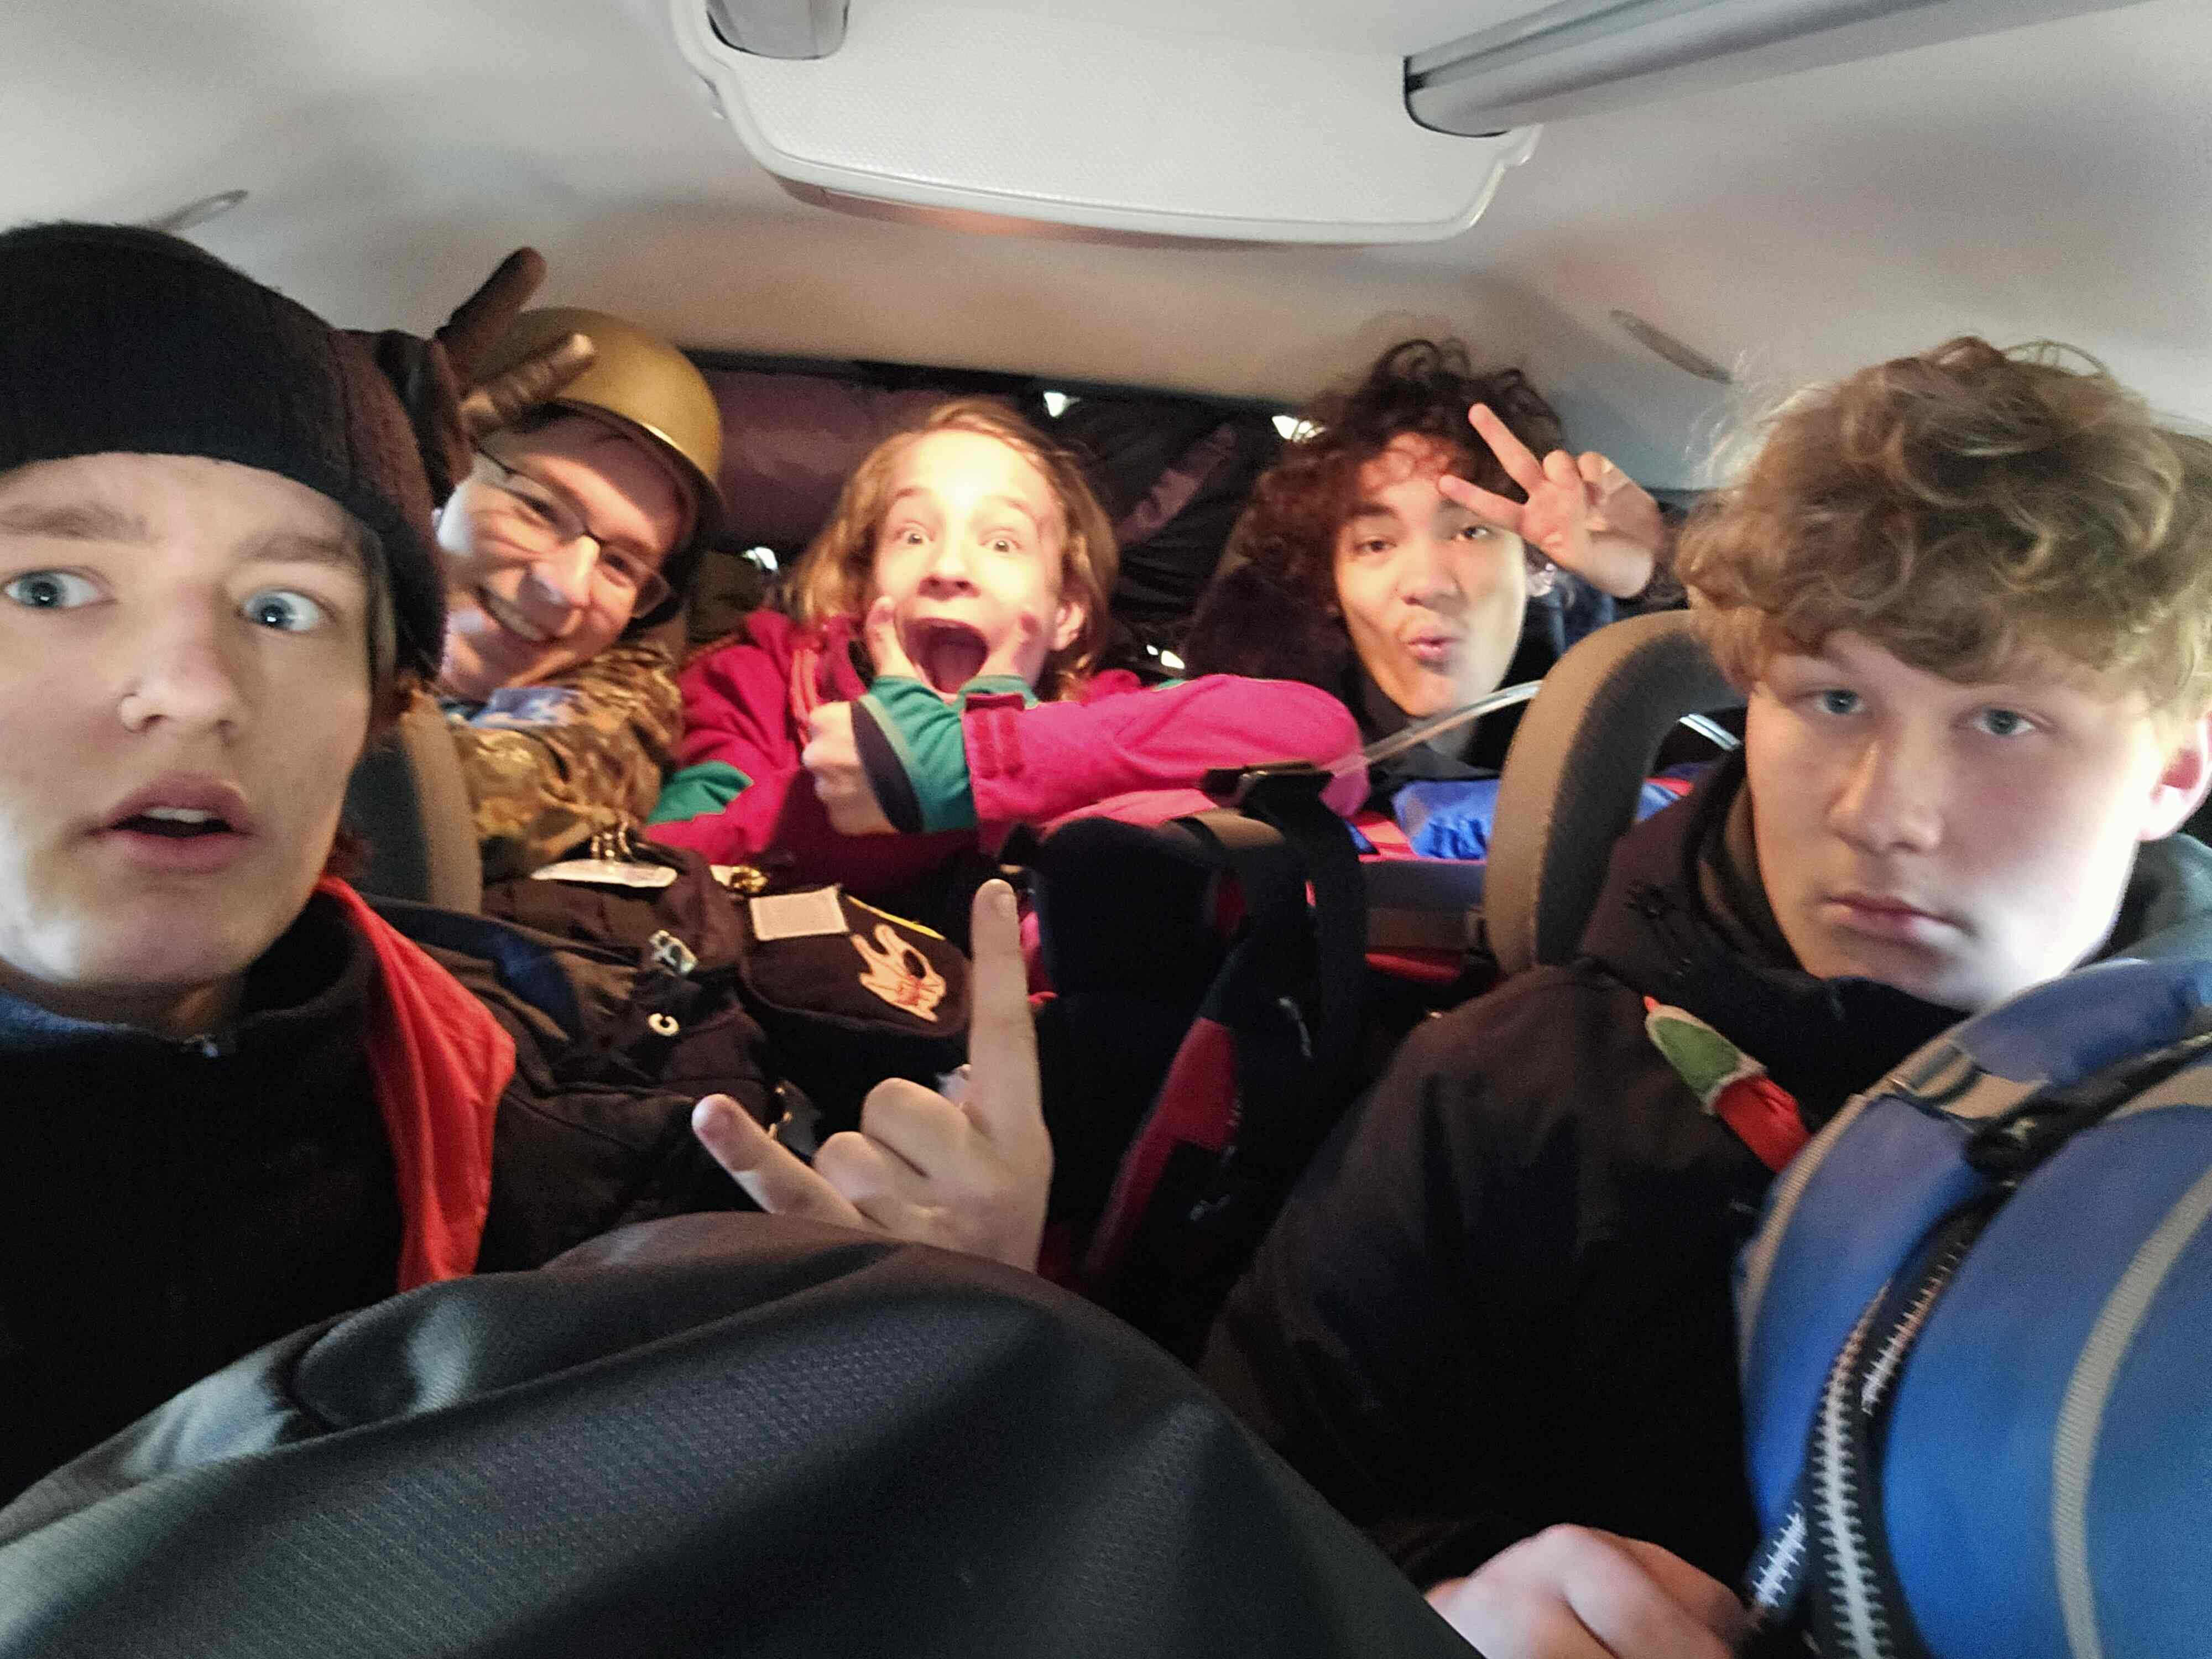
\includegraphics[width=1.0\linewidth]{assets/telttaretki2}

\end{multicols}

\noindent\null\hfill Texti: Päärynä-Hyttyset\\
\noindent\null\hfill Kuvat: PäHy, Leo \& Tanguy\\

